%!TEX root = main.tex
\setcounter{chapter}{5}
\setcounter{section}{3}
\setcounter{theorem}{0}
\setcounter{equation}{0}

\lectureheader{161}{Calculus I}{Definite integrals}{\textit{Thomas' Calculus} \thesection}

\begin{remark}\,
\begin{itemize}
\item Hooke's law says that the force $F$ required to hold a compressed or stretched spring $x$ units from its natural (unstressed) length is proportional to $x$, i.e.,
\begin{equation*}
F=kx
\end{equation*}
for some constant $k$ (measured in force per unit of length).
\item The \textbf{work} done by a \underline{constant} force $F$ on an object as it is displaced $d$ units in a \underline{straight line} in the \underline{direction of the force} is $W=Fd$.
\end{itemize}
\end{remark}

\begin{example}
Consider work required to stretch a spring $1$ meter beyond its natural length if its spring constant is $k=30$ \si{N/m}.
Estimate the work done above and below by partitioning the 1-meter interval into $n$ equal subintervals.
What happens to these estimates as $n\to \infty$.
\end{example}

\newpage

\begin{definition}
Let $f$ be a function defined on the finite-length interval $[a,b]$, and let $P=\{x_0,x_1,\dots, x_n\}$ be a partition of the interval $[a,b]$.
A \textbf{Riemann sum} for $f$ over $P$ is a sum of the form
\begin{equation*}
R = \sum_{k=1}^nf(c_k)\Delta_k,
\end{equation*}
where 
\begin{itemize}
\item $\Delta_k=x_k-x_{k-1}$ for $k=1,\dots, n$, and
\item $c_k\in [x_{k-1}, x_k]$ for $k=1,\dots, n$.
\end{itemize}
\end{definition}

\begin{center}
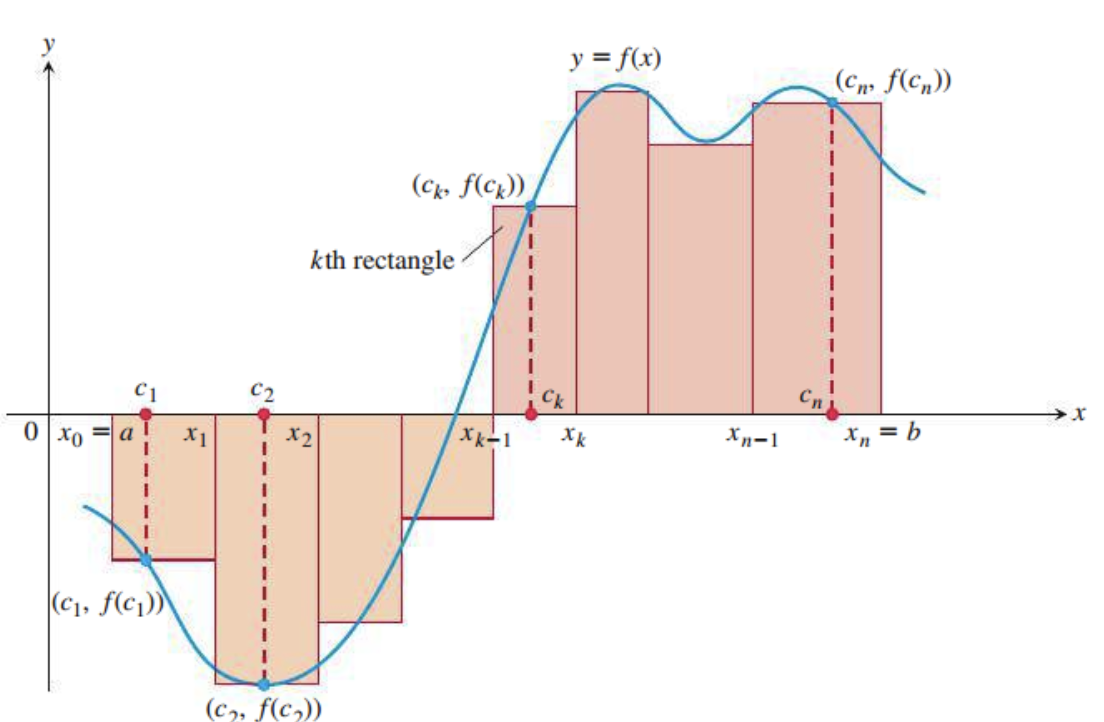
\includegraphics[width=3.5in]{img/riemann_sum}
\end{center}

\begin{definition}
If $P=\{x_0,x_1,\dots, x_n\}$ is a partition, the \textbf{norm of $P$} is 
\begin{equation*}
||P|| = \max\{x_k-x_{k-1} : k=1,\dots, n\}.
\end{equation*}
\end{definition}

\begin{definition}
Let $f$ be a function defined on the finite-length interval $[a,b]$.
We say that $f$ is \textbf{integrable on $[a,b]$} if there is a real number $I$ so that for every $\epsilon>0$, there is a $\delta>0$ so that for every partition $P=\{x_0,x_1,\dots, x_n\}$ with $||P||<\delta$ and every Riemann sum $\DS\sum_{k=1}^nf(c_k)\Delta_k$,
\begin{equation*}
\left|\sum_{k=1}^nf(c_k)\Delta_k - I\right| <\epsilon.
\end{equation*}
If $f$ is integrable, then we say that
\begin{equation*}
\int_a^bf(x)\dee x = I = \lim_{||P||\to 0}\sum_{k=1}^nf(c_k)\Delta_k
\end{equation*}
is the \textbf{definite integral of $f$ over $[a,b]$}.
\end{definition}

\begin{remark}
The symbol chosen for the variable of integration does not matter, e.g.,
\begin{equation*}
\int_a^bf(x)\dee x = \int_a^bf(t)\dee t = \int_a^bf(u)\dee u.
\end{equation*}
\end{remark}

\newpage


\begin{remark}
The definite integral provides a tool for physicists to extend the definition of work to nonconstant forces acting on objects as they move along a 1-dimensional path.
In calc III, we develop tools for higher dimensional paths.
\end{remark}

\begin{definition}
The \textbf{work} done by a variable force $F(x)$ acting on an object in the same or opposite direction of the object as it moves along the $x$-axis from $x=a$ to $x=b$ is
\begin{equation*}
W=\int_a^bF(x)\dee x.
\end{equation*}
\end{definition}

\vfill

\begin{theorem}
If $f$ is continuous  except possibly for at most finitely many jump or removable discontinuities on $[a,b]$, then $f$ is integrable on $[a,b]$.
\end{theorem}
\begin{remark}
In fact, $f$ can even have some infinite discontinuities provided that they are not ``too serious."
Addressing these situations will be one subject of study in calc II.
\end{remark}

\vfill

\begin{remark}
The definite integral also provides a tool for mathematicians to extend the definition of area to objects with curved sides.
In retrospect, when the ancients ``discovered" the formula for the area of a circle with radius $r$, what they really did was ``plausibly define" it to be $\pi r^2$ through a method not unlike the definite integral.
\end{remark}

\begin{definition}
If $f(x)\ge 0$ and integrable on $[a,b]$, then the \textbf{area $A$ under the curve $y=f(x)$} \textbf{over $[a,b]$} is 
\begin{equation*}
A=\int_a^bf(x)\dee x.
\end{equation*}
\end{definition}

\vfill

\newpage

\begin{example}
Compute the area $A$ under $y=x$ over the interval $[a,b]$ as follows.
\begin{enumerate}[label=(\alph*)]
\item Use geometry.
\item Use a definite integral.
\end{enumerate}
\end{example}

\newpage

\begin{example}
Compute the area $A$ under $y=x^2$ over the interval $[a,b]$.
\end{example}

\newpage

\begin{definition}
If $f$ is integral on $[a,b]$, then its \textbf{mean} (or \textbf{average value}) on $[a,b]$ is
\begin{equation*}
\avg(f) = \frac{1}{b-a}\int_a^bf(x)\dee x.
\end{equation*}
\end{definition}

\begin{example}
Compute the average value of $f(x)=\sqrt{4-x^2}$ over the $[-2,2]$.
\end{example}

\newpage

\begin{definition}
If $a\le b$, then 
\begin{align*}
\int_a^af(x)\dee x&=0,\\
\int_b^af(x)\dee x&=-\int_a^bf(x)\dee x.
\end{align*}
\end{definition}

\vfill

\begin{theorem}[Additivity]
If $f$ is integrable on $[a,b]$ and on $[b,c]$, then
\begin{equation*}
\int_a^cf(x)\dee x = \int_a^bf(x)\dee x + \int_b^cf(x)\dee x
\end{equation*}
\end{theorem}

\vfill

\begin{theorem}[Linearity]
If $f$ and $g$ are integrable on $[a,b]$ and $c,d\in\R$, then
\begin{equation*}
\int_a^b\big(cf(x)+dg(x)\big)\dee x = c\int_a^bf(x)\dee x + d\int_a^bg(x)\dee x.
\end{equation*}
\end{theorem}

\vfill

\begin{theorem}[Domination]
If $f$ and $g$ are integrable on $[a,b]$ and $f(x)\ge g(x)$ for all $x\in [a,b]$, then
\begin{equation*}
\int_a^bf(x)\dee x\ge \int_a^bg(x)\dee x.
\end{equation*}
\end{theorem}

\vfill

\newpage

\begin{example}
To evaluate $\DS\int_0^1\sqrt{1+\cos x}\dee x$ we require methods from calc II.
Nevertheless, we know that it exists.  Why?
Find upper and lower bounds on the integral.
\end{example}

